\subsubsection{\texttt{RF-3}: anonimato de propuestas de estudiantes}
\label{subsec:rf3}

Cuando un profesor descargaba un ejercicio en las primeras versiones de \textit{VSCode4Teaching}, la estructura de ficheros que se habilitaba en su entorno de desarrollo incluía un directorio ``template'' con la plantilla original del ejercicio y tantos directorios como propuestas de alumnos terminadas o parcialmente guardadas hubiese, identificando cada una de ellas con el nombre de usuario del alumno. Además, el \textit{dashboard} ---creado para que los profesores pudieran obtener información del progreso de sus estudiantes en la realización de los ejercicios--- incluía como elemento principal una tabla que reflejaba nombre, apellidos, nombre de usuario y fecha de última modificación para cada uno de los estudiantes del curso.

En cumplimiento del primer objetivo de los recogidos en el \referenciaCapitulo{cap:objetivos}, la presente tarea conduce a la modificación de los mecanismos de identificación de las propuestas de resolución de los ejercicios remitidas por los estudiantes con el fin de poder garantizar su anonimato. Para ello, se introducen dos requisitos derivados:

\begin{itemize}
    \item El requisito \texttt{RF-3.1} establece la necesidad de alterar el sistema de nomenclatura que se emplea para almacenar las propuestas enviadas por los estudiantes. Como consecuencia, se introduce una modificación por la que el servidor asigna como nombre del directorio de cada una de ellas un texto del formato ``student\_\texttt X'', siendo \texttt X el número identificador de la propuesta almacenado en base de datos. Este formato permite cotejar el número empleado para formar el nombre del directorio (\texttt X) con los datos persistidos, pudiendo así relacionar la propuesta de cada estudiante con su propia información de forma rápida. La \referenciaFigura{fig:reqf3-1} recoge una comparativa entre los formatos anterior y actual.
    \item El requisito \texttt{RF-3.2} estipula las dos actuaciones que se ejecutan sobre el \textit{dashboard}: la modificación de la columna que recoge el nombre de usuario de los estudiantes, introduciendo en ella el nombre del directorio que recoge su propuesta de solución; y la introducción de un elemento de control interactivo que permita a los docentes ocultar o mostrar la columna de nombres y apellidos a elección. En la \referenciaFigura{fig:reqf3-2} se destaca este elemento de control y se puede visualizar la tabla sin y con la mencionada columna cuando este está activado y desactivado, respectivamente.
\end{itemize}

De este modo, la ejecución de ambos requisitos permite lograr una situación de total anonimato de los estudiantes si así lo desea el docente, pudiendo relacionar cada nombre de directorio con el nombre propio y los apellidos de cada estudiante en el \textit{dashboard} cuando lo desee.

\begin{figure}[ht]
    \centering
    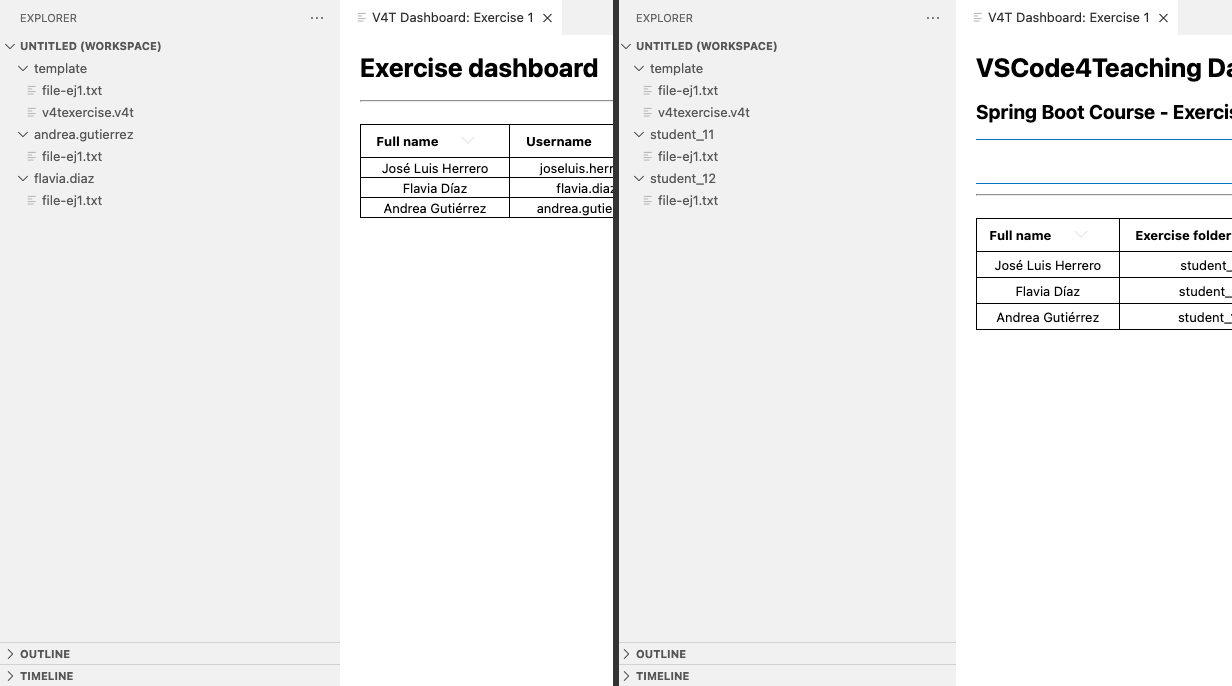
\includegraphics[width=\textwidth]{imagenes/utilizadas/4-3-implementacion/rf3-1.png}
    \caption{Comparativa entre los formatos anterior (izquierda) y actual (derecha) de almacenamiento de propuestas de estudiantes.}
    \label{fig:reqf3-1}
\end{figure}

\begin{figure}[ht]
    \centering
    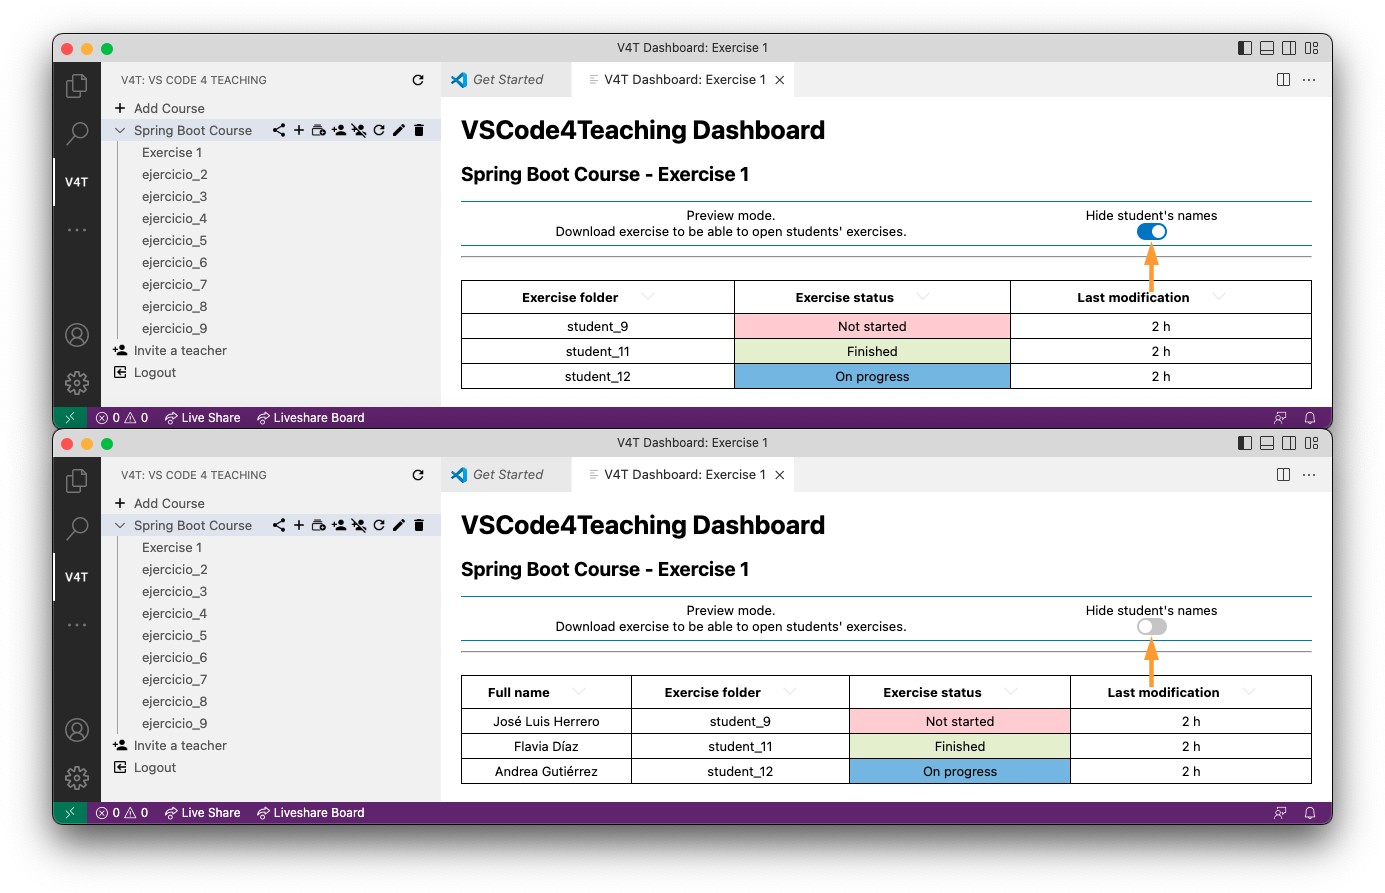
\includegraphics[width=0.975\textwidth]{imagenes/utilizadas/4-3-implementacion/rf3-2.png}
    \caption{Captura de la extensión en la que se destaca el nuevo elemento para ocultar y mostrar la identidad de los estudiantes.}
    \label{fig:reqf3-2}
\end{figure}
